\section{Introduction}

Any compiler includes a recognition algorithm which is essentially a finite automaton enriched with an auxiliary memory organized as a pushdown or LIFO stack of 
unbounded capacity, which stores the symbols. The input or source string, delimited on the right end by an end-marker $\dashv$, is: 
\[a_1a_2\dots a_i\dots a_n\dashv\]
The following operations apply to a stack:
\begin{itemize}
    \item Push: places the symbol(s) onto the stack top. 
    \item Pop: removes symbol from the stack top, if the stack is not empty; otherwise reads $Z_0$. 
    \item Stack emptiness test: true if the stack is empty, false otherwise. 
\end{itemize}
The symbol $Z_0$ is the stack bottom and can be read but not removed. At each instant the machine configuration is specified by: the remaining portion of the input 
string still to be read, the current state, and the stack contents. With a move the pushdown automaton: 
\begin{itemize}
    \item Reads the current character and shifts the input head, or performs a spontaneous move without shifting the input head. 
    \item Reads the stack top symbol and removes it from the top if the stack is not empty, or reads the stack symbol $Z_0$ if the stack is empty. 
    \item Depending on the current character, state and stack top symbol, it goes into the next state and places none, one or more symbols onto the stack top. 
\end{itemize}
\begin{definition}
    A pushdown automaton $M$ is defined by:
    \begin{itemize}
        \item $Q$ a finite set of states of the control unit.
        \item $\Sigma$ a finite input alphabet.
        \item $\Gamma$ a finite stack alphabet.
        \item $\delta$ a transition function.
        \item $q_0 \in Q$ the initial state.
        \item $Z_0 \in \Gamma$ the initial stack symbol.
        \item $F \subseteq Q$ a set of final states.
    \end{itemize}
\end{definition}
The domain and range of the transition function are made of Cartesian products:
\begin{itemize}
    \item Domain: $Q \times \left(\Sigma \cup \{\varepsilon\}\right) \times \Gamma$. 
    \item Range: the set of the subsets of $Q \times \Gamma^{*}$. 
\end{itemize}
The possible moves are: 
\begin{itemize}
    \item Reading move: in the state $q$ with symbol $Z_0$ on the stack top, the automaton reads char $a$ and enters one of the states $p_i$ with $1 \leq i \leq n$, 
        after orderly executing the operations pop and push ($\gamma_i$): 
        \[\delta(q,a,Z)=\{(p_1,\gamma_1), (p_2,\gamma_2),\dots,(pn,\gamma_n)\}\]
    \item Spontaneous move: in the state $q$ with symbol $Z_0$ on the stack top, the automaton does not read any input character and enters one of the states $p_i$
        with $1 \leq i \leq n$, after orderly executing the operations pop and push ($\gamma_i$): 
        \[\delta(q,\varepsilon,Z)=\{(p1,\gamma_1), (p2,\gamma_2),\dots,(pn,\gamma_n)\}\]
\end{itemize}
There is non-determinism: for a triple (state, input, stack top) there are two or more possible moves that consume none or one input character. 
\begin{definition}
    The \emph{instantaneous configuration} of a machine $M$ is a 3-tuple: 
    \[(q,y,\eta)\in Q \times \Gamma^{*} \times \Gamma^{+}\]
    which specifies:
    \begin{itemize}
        \item $q$, the current state,
        \item $y$, the remaining portion (suffix) of the source string $x$ to be read.
        \item $\eta$, the stack content.
    \end{itemize}

    The \emph{initial} configuration of machine $M$ is: 
    \[(q_0,x,Z_0)\]

    The \emph{final} configuration of machine $M$ is: 
    \[(q,\varepsilon,\lambda)\]
\end{definition}
Applying a move, a transition from a configuration to another occurs, to be denoted as: 
\[(q,y,\eta)\rightarrow(p,z,\lambda)\]
Note that a chain of one or more transitions is denoted by $\rightarrow^{+}$. An input string $x$ is accepted by final state if there is the following computation
\[(q_0,x,Z_0)\mapsto^{*}(q,\varepsilon,\lambda)\]
where $q \in F$ and $\lambda\in\Gamma^{*}$, whereas there is not any specific condition for $\lambda$; sometimes $\lambda$ happens to be the empty string, but this 
is not necessary. 

\subsection*{State-transition diagram for PDA}
The transition function of a finite automaton can be graphically presented, although its readability is somewhat lessened by the need to specify stack operations.
\begin{example}
    The language $L=\{uu^R|u \in \{a,b\}^{*}\}$ of the palindromes of even length is accepted with final state by the pushdown recognizer. 
    \begin{figure}[H]
        \centering
        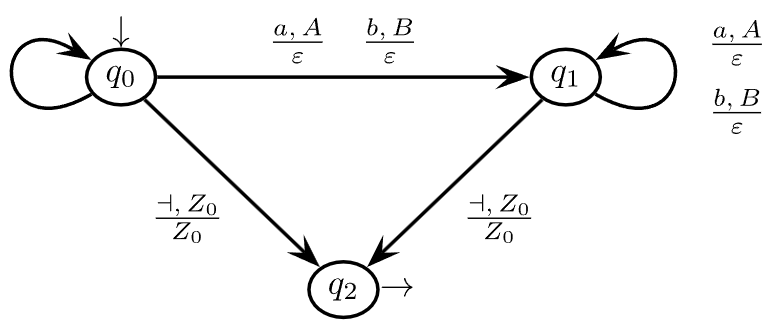
\includegraphics[width=0.5\linewidth]{images/PDA.png}
    \end{figure}
\end{example}

\subsection*{From a grammar to a PDA}
Grammar rules can be viewed as the instructions of a non-deterministic pushdown automaton. Intuitively such an automaton works in a goal-oriented way and uses the 
stack as a notebook of the sequence of actions to undertake in the next future. The stack symbols can be both terminals and non-terminals of the grammar. If the
stack contains the symbol sequence $A_1 \dots A_k$, then the automaton executes first the action associated with $A_k$, which should recognize if in the input string 
from the position of the current character $a_i$ there is a string w that can be derived from $A_k$; if it is so, then the action shifts the input head of 
$\left\lvert w\right\rvert $ positions. An action can be recursively divided into a series of sub-actions, if to recognize the non-terminal symbol $A_k$ it is 
necessary to recognize other non-terminals. 

The initial action is the grammar axiom: the pushdown recognizer must check if the source string can be derived from the axiom. Initially the stack contains
only the symbol $Z_0$ and the axiom $S$, and the input head is positioned on the initial character of the input string. At every step the automaton
chooses (non-deterministically) one applicable grammar rule and executes the corresponding move. The input string is recognized accepted when,
and only when, it is completely scanned and the stack is empty. 
\begin{figure}[H]
    \centering
    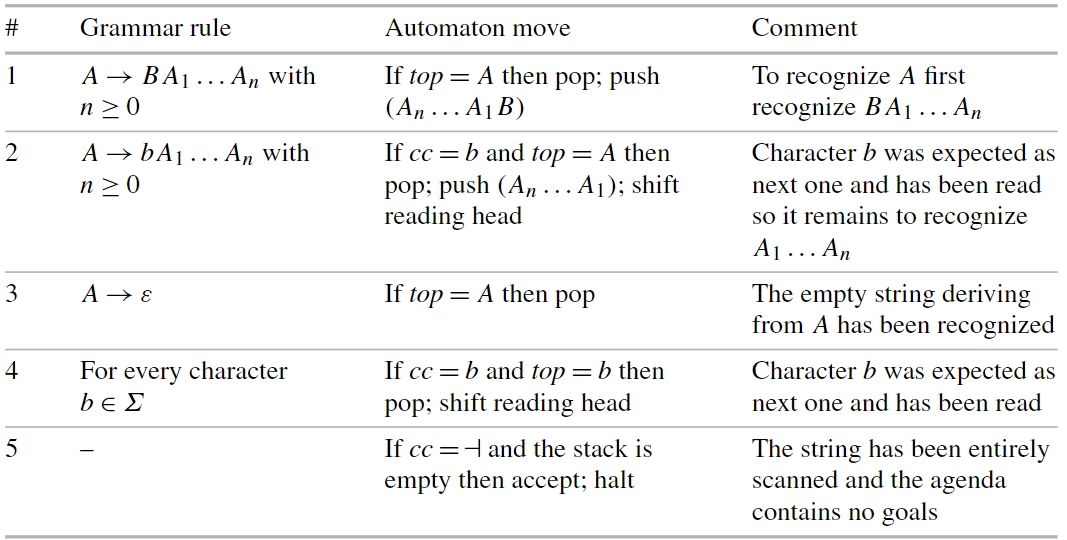
\includegraphics[width=1\linewidth]{images/gramPDA.png}
    \caption{Correspondence between a grammar and a PDA}
\end{figure}

The family of free languages generated by free grammars coincides with the family of the languages recognized by one-state pushdown automata. 

Unfortunately in general the resulting pushdown automaton is non-deterministic, as it explores all the moves applicable at any point and has an exponential time
complexity with respect to the length of the source string. There are more efficient algorithms. 

\subsection*{Varieties of pushdown automata}
The acceptance modes can be: 
\begin{enumerate}
    \item By final state: accepts when enters a final state independently of the stack contents. 
    \item By empty stack: accepts when the stack gets empty independently of the current state. 
    \item Combined: by final state and empty stack.
\end{enumerate}
For the family of (non-deterministic) pushdown automata with states, the three acceptance modes listed above are equivalent. 

A generic pushdown automaton may execute an unlimited number of moves without reading any input character. This happens if, and only if, it enters a loop made only
of spontaneous moves. Such a behaviour prevents it of completely reading the input string, or causes it to execute an unlimited number of moves before deciding whether
to accept or reject the string. Both behaviours are undesirable in the practice. It is always possible to build an equivalent automaton with no spontaneous loops. 

A pushdown automaton operates in on-line mode if it decides whether to accept or reject the string as soon as it reads the last character of the input string, and
then it does not execute any other move. Clearly from a practical perspective the on-line mode is a desirable behavior. It is always possible to build an equivalent 
automaton that works in on-line mode. 

\subsection*{One family for context-free languages and PDA}
The family CF of context-free languages coincides with that of the languages recognized by unrestricted pushdown automata. 

And more specifically the family CF of (context-) free languages coincides with that of the languages recognized by the one-state non-deterministic pushdown automata.

\subsection*{Intersection of regular and free languages}
It is easy to justify that the intersection of a free and a regular language is free as well. Given a grammar $G$ and a finite state automaton $A$, the pushdown 
automaton $M$ that recognizes the intersection $L(G) \cap L(A)$ can be obtained as follows: 
\begin{enumerate}
    \item Construct the one-state pushdown automaton $N$ that recognizes $L (G)$ by empty stack. 
    \item Construct the pushdown automaton $M$ (with states), the state-transition graph of which is. The Cartesian product of those of $N$ and $A$, by the Cartesian 
        product construction so that the actions of $M$ on the stack are the same as those of $N$. 
\end{enumerate}
The obtained pushdown automaton $M$: 
\begin{enumerate}
    \item As its states, has pairs of states of the component machines $N$ and $A$. 
    \item Accepts by final state and empty stack (combined acceptance mode). 
    \item The states that contain a final state of $A$ are themselves final. 
    \item Is deterministic, if both component machines $N$ and $A$ are so. 
    \item Accepts by final state all and only the strings that belong to the intersection language.
\end{enumerate}
\begin{example}
    The intersection of the automaton is: 
    \begin{figure}[H]
        \centering
        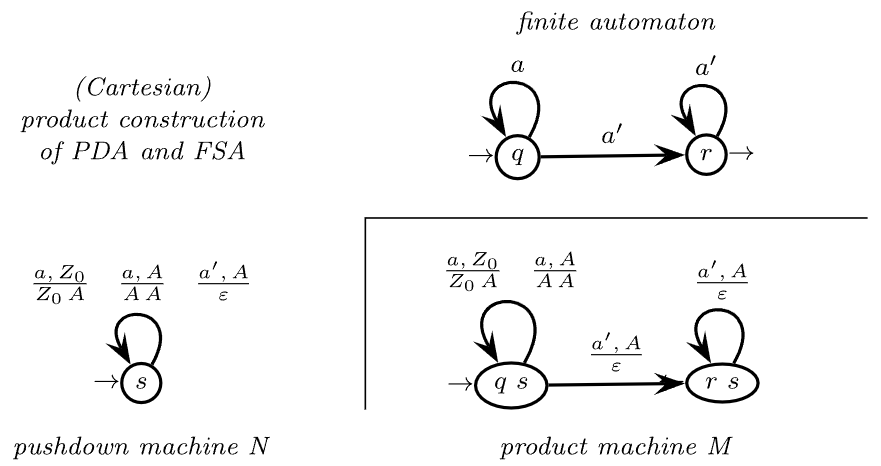
\includegraphics[width=0.9\linewidth]{images/PDAint.png}
    \end{figure}
\end{example}